\chapter{Simulation Experiments}

Knowing that real-robot experiments are expensive and error-prone, we developed a simulation in Mujoco as a test bed for our algorithms. In simulation, we can also access data that is not accessible in the real world, scale up demonstrations quickly, and have a controlled environment with reproducibility to test new methods. In the following sections, the tasks used for evaluation are introduced, and the results are presented and discussed. 

\section{Tasks}

The first environment is a door in a hallway. It contains two tasks: opening the door and walking through the door. For the first task, the robot needs to grab the handle, turn it, and push the door open. Partial success is defined by the robot grasping the handle. This is a relatively easy task involing single-arm manipulation. The second task is a loco-manipulation task, where the robot needs to walk forward while pushing the door open. Partial success is given if the robot opens the door but doesn't walk through it. The initial pose of the robot is randomized based on a normal distribution for both tasks, with a standard deviation of 2 centimeters for the position and .07 radians for the orientation. 

The second environment is a kitchen with two tasks: moving a pot and placing a lid. The first task is a loco-manipulation task requiring the robot to lift up a pot with two hands, walk a step towards a stove, and put the pot on the stove. Partial success is granted for lifting the pot. For the second task, the robot should grab the lid next to the pot and put it on the pot. Grasping the lid constitutes a partial success. This task requires precision. The positions of the pot, stove, and lid are randomized along with the initial pose of the robot. The stove's position is uniformly distributed from -5 to 5 centimeters, while the pot and lid are placed from -3 to 3 centimeters away from the stove. The pot and lid are made to be light since the robot dynamic model currently does not consider external forces. 

We collected 200 demonstrations for each of the 4 tasks. The neural network architecture and training are identical to those introduced in Chapter 4. 

\section{Results}

The evaluation results for each task are presented in Table \ref{table:results}. Image sequences of successful episodes are presented in Figure \ref{figure:sim-eval}. 

\begin{table}[ht]
	\centering
	\begin{tabular}{|c|c|c|c|}
		\hline
		& Success & Partial success & Fail\\
		\hline
		Open door & 80\% & 13 \% & 7\% \\
		\hline
		Walk through door & 74 \% & 13\% & 13\%\\
		\hline
		Moving pot & 8 \% & 53 \% & 40\%\\
		\hline
		Move lid & 8 \% & 53 \% & 40 \%\\
		\hline
	\end{tabular}
	\caption{The evaluation success rates on the 4 simulation tasks.}
	\label{table:results}
\end{table}

A common failure mode for the pot task is the robot falling down when moving the pot. When the robot is side-stepping, the robot's arms tend to swing sideways to maintain balance. However, if the robot is holding the pot with two hands, the frictions on the pot handle constrain the arm motion. After lifting the pot, if the hands are not kept steady during side-stepping, the robot can easily fall. 

The low success rate for moving the lid can be explained by the precision needed to grasp the lid's handle, which requires inserting the robot's gripper below the handle and above that lid. Also, when the lid is being put on the pot, occlusion occurs since the robot's arm is blocking the view of the pot. When the robot's arms are made invisible, we found that the success rate is 10\% higher. 

Similar to the hardware experiments, we hypothesize that the whole-body controller tracking error is partially responsible for the imprecise manipulation. It's also not clear if the model is able to successfully extract depth information from the stereoscopic images. SimNet \cite{kollar2021simnet} demonstrates that this is indeed possible, but they're using a stereo matching neural network crafted specifically for the purpose of extracting depth information, whereas we are simply training a ResNet in an end-to-end manner directly on the downstream task.

\begin{figure}
	\centering
	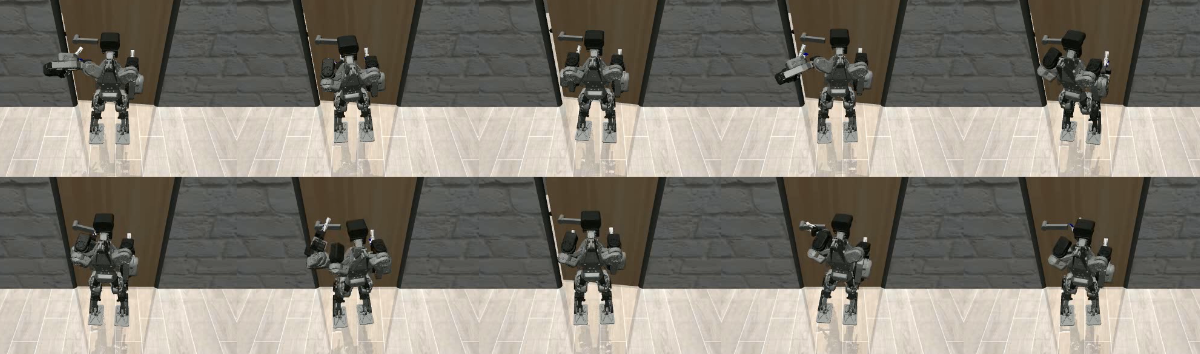
\includegraphics[width=.95\linewidth]{door1.png}\\
	\vspace{1em}             
	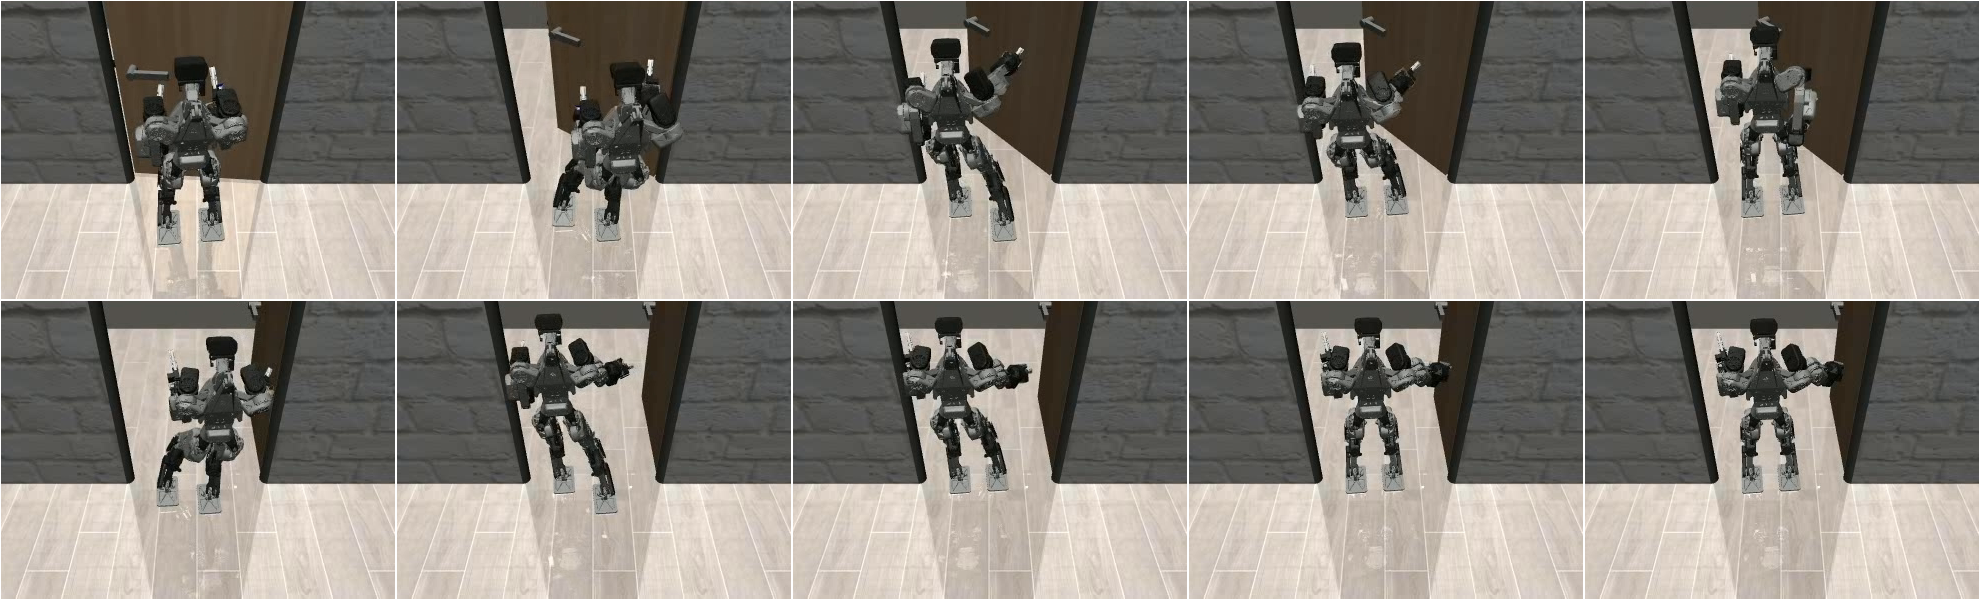
\includegraphics[width=.95\linewidth ]{door2.png}\\
	\vspace{1em}             
	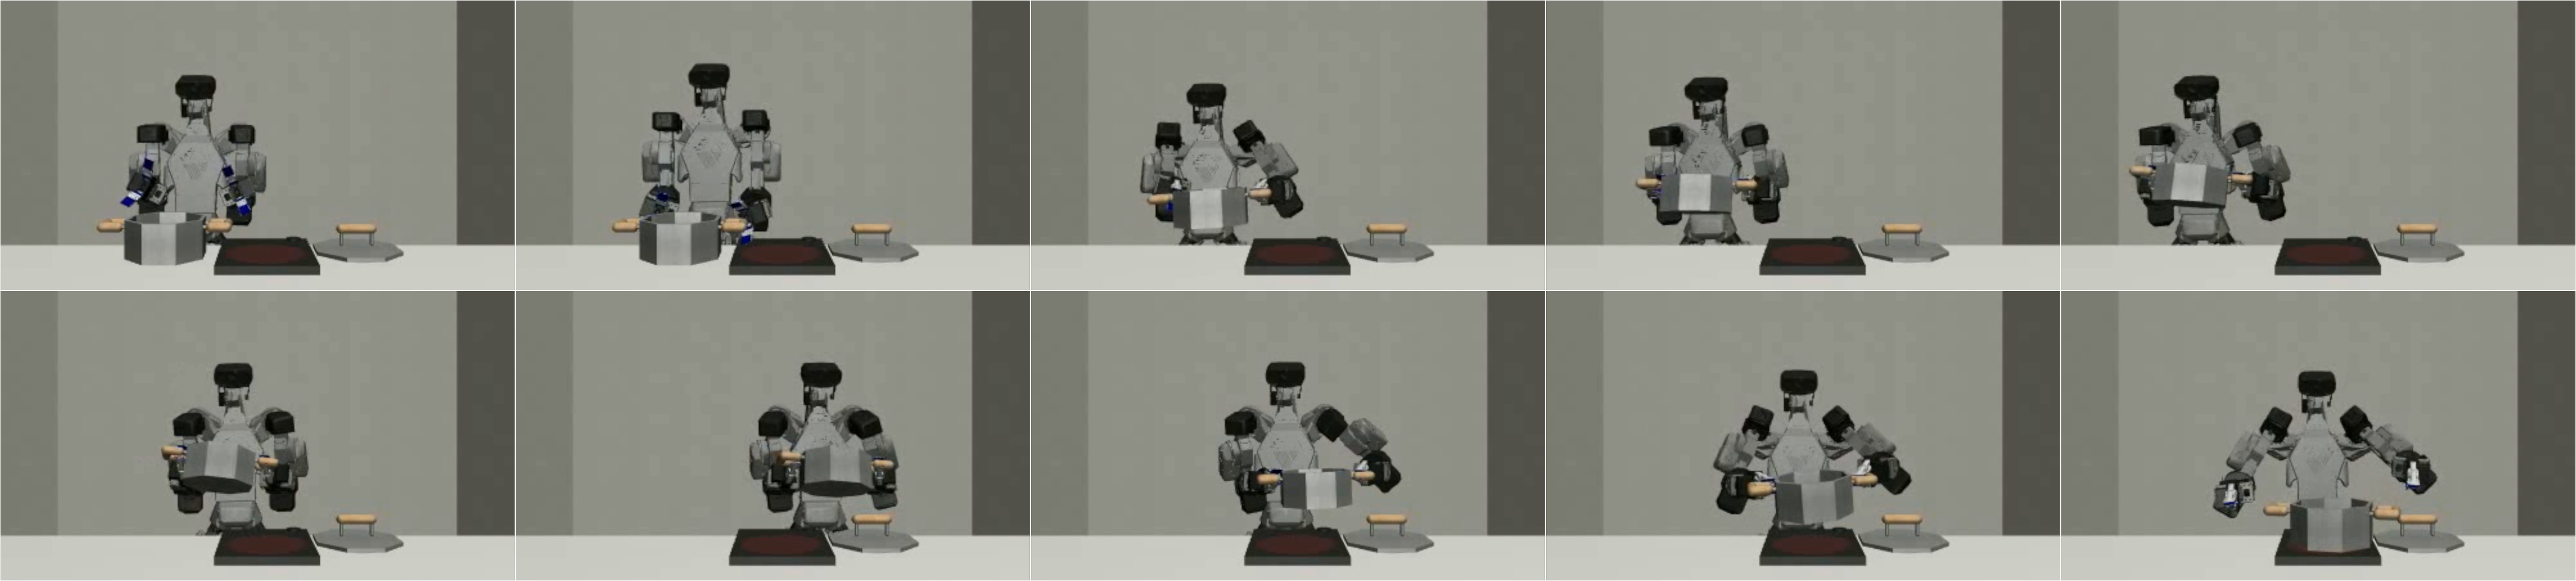
\includegraphics[width=.95\linewidth ]{pot.png}\\
	\vspace{1em}             
	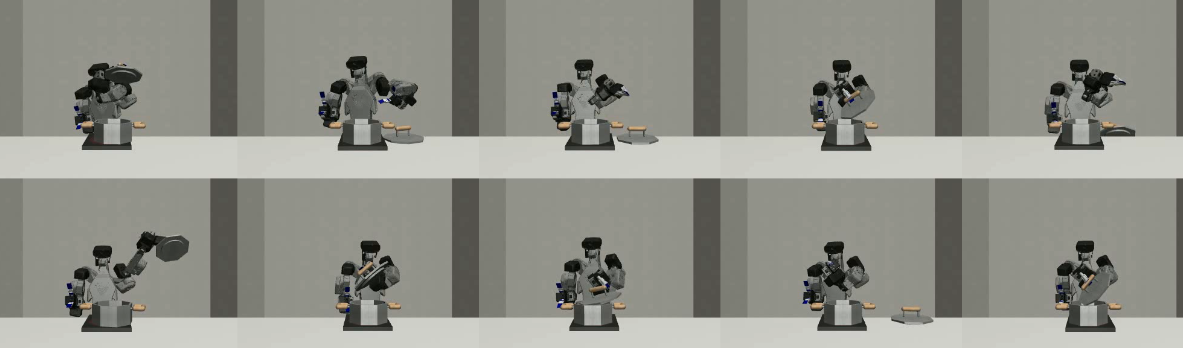
\includegraphics[width=.95\linewidth ]{lid.png}
	\caption{A successful episode from each simulation task. From top to bottom, we have opening the door, pushing the door, moving the pot, and placing the lid. The $2 \times 5$ image sequences are read from left to right and top to bottom. Note that the robot swings laterally when performing locomotion. }
	\label{figure:sim-eval}
\end{figure}
